\documentclass[10pt]{article}
\usepackage[margin=0.56in]{geometry}
\usepackage{amsmath,amssymb,booktabs,graphicx,microtype,xcolor}

\usepackage[hidelinks]{hyperref}
\setlength{\parindent}{0pt}
\setlength{\parskip}{3pt}
\setlength{\abovedisplayskip}{3pt}
\setlength{\belowdisplayskip}{3pt}
\setlength{\textfloatsep}{5pt}
\renewcommand{\arraystretch}{1.08}

\title{\vspace{-1.15cm}\textbf{Two-Block Circuit Formation under Langevin Annealing:\\Stationary Theory versus Training}}
\author{}
\date{\vspace{-1.3cm}}

\begin{document}
\maketitle
\vspace{-0.75cm}

\textbf{Result in one sentence.}
Annealed Langevin noise at $T_0=10^{-7}$ does not change which circuit training selects (joint
training still settles in the direct phase $H_D$, parent-warm in the compositional phase $H_C$),
and picking the lower-objective run per cell gives $H_C$ in only 29 of the theory's 47 cells.

\textbf{Experiment.}
Same objective, network (bias-free two-block ReLU, $N=1024$, float64, exact four-bit cube,
$\gamma_2=\gamma_4=2$) and $8\times9$ decay grid as the deterministic report
($\lambda_E=\lambda_2=\lambda_p=\lambda_4=\lambda_0$, $\lambda_1=(\lambda_1/\lambda_2)\lambda_0$),
seed 0, both protocols.  The final phase is plain SGD (momentum 0) with Langevin noise added
after every update, $\Delta\theta=\sqrt{2\eta_g T(t)}\,\xi$, $\xi\sim\mathcal N(0,I)$, using each
optimizer group's rate ($\eta_{E,V}=10^{-2}$, readout $\eta_W=10^{-2}/N$), so the stationary
density is $\propto e^{-J/T}$.  $T=T_0$ for 5k steps, decays exponentially to $10^{-3}T_0$ over
25k steps, and is 0 for the last 20k; every cell runs exactly 50k steps.  Parent-warm cells start
from the deterministic sweep's own seed-0 warm starts (noise-free pretraining, momentum 0.9).

\textbf{New measurements.}  A block-2 neuron is a $2{+}2{\to}4$ unit when $\ge 90\%$ of
$\mathrm{Var}\,z_n$ lies on the parent modes $x_0x_1$, $x_2x_3$ with balance
$\min/\max\ge0.8$, and it produces the quad mode with $|a_n|\ge10^{-6}$ (units below this on every
target mode are dead).  With $a_n$ the neuron's $d4$ amplitude and $w_{4,n}$ its readout weight,
\[
\varphi_{\rm out}=\frac{\sum_{2+2\to4}|w_{4,n}a_n|}{\sum_{\rm block\,2}|w_{4,n}a_n|},\qquad
\varphi_{\rm sq}=\frac{\sum_{2+2\to4}a_n^2}{\sum_{\rm block\,2}a_n^2},\qquad
f_C^{\,\rm sq}=\frac{\sum_{\rm block\,2}a_n^2\,\pi_n}{\sum_{\rm block\,1}a_n^2+\sum_{\rm block\,2}a_n^2},
\]
where $\pi_n$ is the parent share of $\mathrm{Var}\,z_n$ (the weight $f_C$ uses).  Theory:
$\varphi=1$ in $H_C$, 0 otherwise.

\begin{center}
\small\setlength{\tabcolsep}{4pt}
\begin{tabular}{@{}lcccccc@{}}
\toprule
 & \multicolumn{2}{c}{Parent-warm} & \multicolumn{2}{c}{Joint} & \multicolumn{2}{c}{Lower objective} \\
Seed 0, $8\times9$ grid & determ. & annealed & determ. & annealed & determ. & annealed \\
\midrule
Phase agreement with theory & 87.5\% & 79.2\% & 37.5\% & 36.1\% & 75.0\% & 72.2\% \\
Gate $H_C\Leftrightarrow R>1/\sqrt8$ (active cells) & 89.5\% & 96.2\% & 49.1\% & 34.0\% & 94.7\% & 83.0\% \\
Mean $|f_C-f_C^{\rm theory}|$ & 0.147 & 0.162 & 0.340 & 0.350 & 0.199 & 0.186 \\
Cells in $H_C$ (theory: 47) & 46 & 48 & 3 & 3 & 29 & 29 \\
Cells won (parent-warm / joint) & & & & & 30/42 & 33/39 \\
\midrule
Protocols select different phases & \multicolumn{6}{c}{44/72 cells (deterministic) $\to$ 48/72 cells (annealed)} \\
\bottomrule
\end{tabular}
\end{center}

\textbf{Observations.}
(i) \emph{Basin selection is unchanged.}  Joint training keeps $H_D$ in every cell where it
had it except two; parent-warm changes 8 cells.  Three move $H_D\to H_C$ inside the theory's
$H_D$ region ($\lambda_1/\lambda_2=20$ at $\lambda_0\le3\times10^{-4}$, and $(10^{-2},5)$), which
lowers phase agreement even though the measured-$R$ gate now predicts the parent-warm phase in
96\% of active cells.  Five strong-decay cells ($\lambda_0=0.1$--$0.3$) end as
\emph{parents\_only}: their $d4$ amplitude is still rising at 50k steps ($A_4=0.005$--$0.22$),
whereas four of them reached $A_4=0.63$--$0.78$ with momentum 0.9 (the fifth was suppressed).
Momentum-free SGD moves $\sim10\times$ more slowly, so these cells are unfinished rather than
noise-destroyed.
(ii) \emph{Where $H_C$ forms, theory matches at moderate decay.}  The largest parent-warm share,
$f_C=0.738$ at $(\lambda_0,\lambda_1/\lambda_2)=(10^{-2},1)$, sits next to the predicted 0.749.  At
$\lambda_0\le3\times10^{-4}$, however, $f_C=0.46$--$0.49$ regardless of the ratio, whereas the
theory predicts 0.49--0.78 rising with the ratio.
(iii) \emph{Block 2 is compositional only once decay prunes it.}  Inside the theory's $H_C$
region the parent-warm $\varphi_{\rm out}$ grows with $\lambda_0$: 0.44, 0.47, 0.55, 0.72 at
$\lambda_0=10^{-4},3\times10^{-4},10^{-3},3\times10^{-3}$, then 0.80--0.89 for
$\lambda_0\ge10^{-2}$ (theory: 1).  At weak decay half of block 2's $d4$ output comes from
mixed or raw-bit neurons.  In $H_D$ cells $\varphi_{\rm out}\approx0$, as predicted.
(iv) \emph{Output-weighted and block-intrinsic shares agree.}  Across cells
$\mathrm{corr}(\varphi_{\rm out},\varphi_{\rm sq})=0.99$ and $\mathrm{corr}(f_C,f_C^{\rm sq})=0.99$; the
readout-free values are higher at weak decay ($f_C^{\rm sq}\approx0.60$, $\varphi_{\rm sq}\approx0.53$),
so the readout slightly favours the non-compositional routes there, and they converge for
$\lambda_0\ge10^{-2}$ (Fig.~2).
(v) \emph{The lower-objective run is often $H_D$ where theory predicts $H_C$} (Fig.~1, bottom
row).  Of the 18 such cells, 7 at $\lambda_0\le10^{-3}$ are near-ties (joint's $H_D$ is lower by
0.02--0.3\% of $J$); 5 at $\lambda_0=10^{-2}$--$0.1$, $\lambda_1/\lambda_2=0.5$--2 favour $H_D$ by
0.8--8\%, a genuine discrepancy at least with the $H_C$ minima that training reaches; and 6
strong-decay cells are unfinished in both runs.  The selected $H_C$ region is the
low-ratio band plus a wedge up to $\lambda_1/\lambda_2\approx1$--2 at
$\lambda_0=10^{-3}$--$3\times10^{-2}$; the deterministic runs give the same count (29).
(vi) \emph{Losses do not discriminate the phases.}  Final MSE is set mainly by $\lambda_0$ (below
$10^{-5}$ at $\lambda_0=10^{-4}$, $10^{-3}$--$10^{-1}$ at $\lambda_0=0.1$, and 1 where the target is
lost) and is nearly identical for the two protocols (Fig.~3): $H_C$ and $H_D$ fit equally well, so
the circuit is selected by the regularizer and the dynamics, not by the data fit.

\textbf{Limits.}  One seed and a single temperature.  $T_0=10^{-7}$ is $10^3$--$10^6$ times
smaller than the objective differences between the two protocols' minima in the deterministic
sweep ($10^{-4}$--$10^{-1}$), and no joint cell left $H_D$, so at this temperature the noise only
explores within a basin.  The fixed 50k plain-SGD steps also leave the strongest-decay cells
unfinished.  The next tests are a $T_0$ sweep (or a longer hold) and enough noise-free steps for
strong-decay cells to converge.

\begin{figure}[p]
\centering
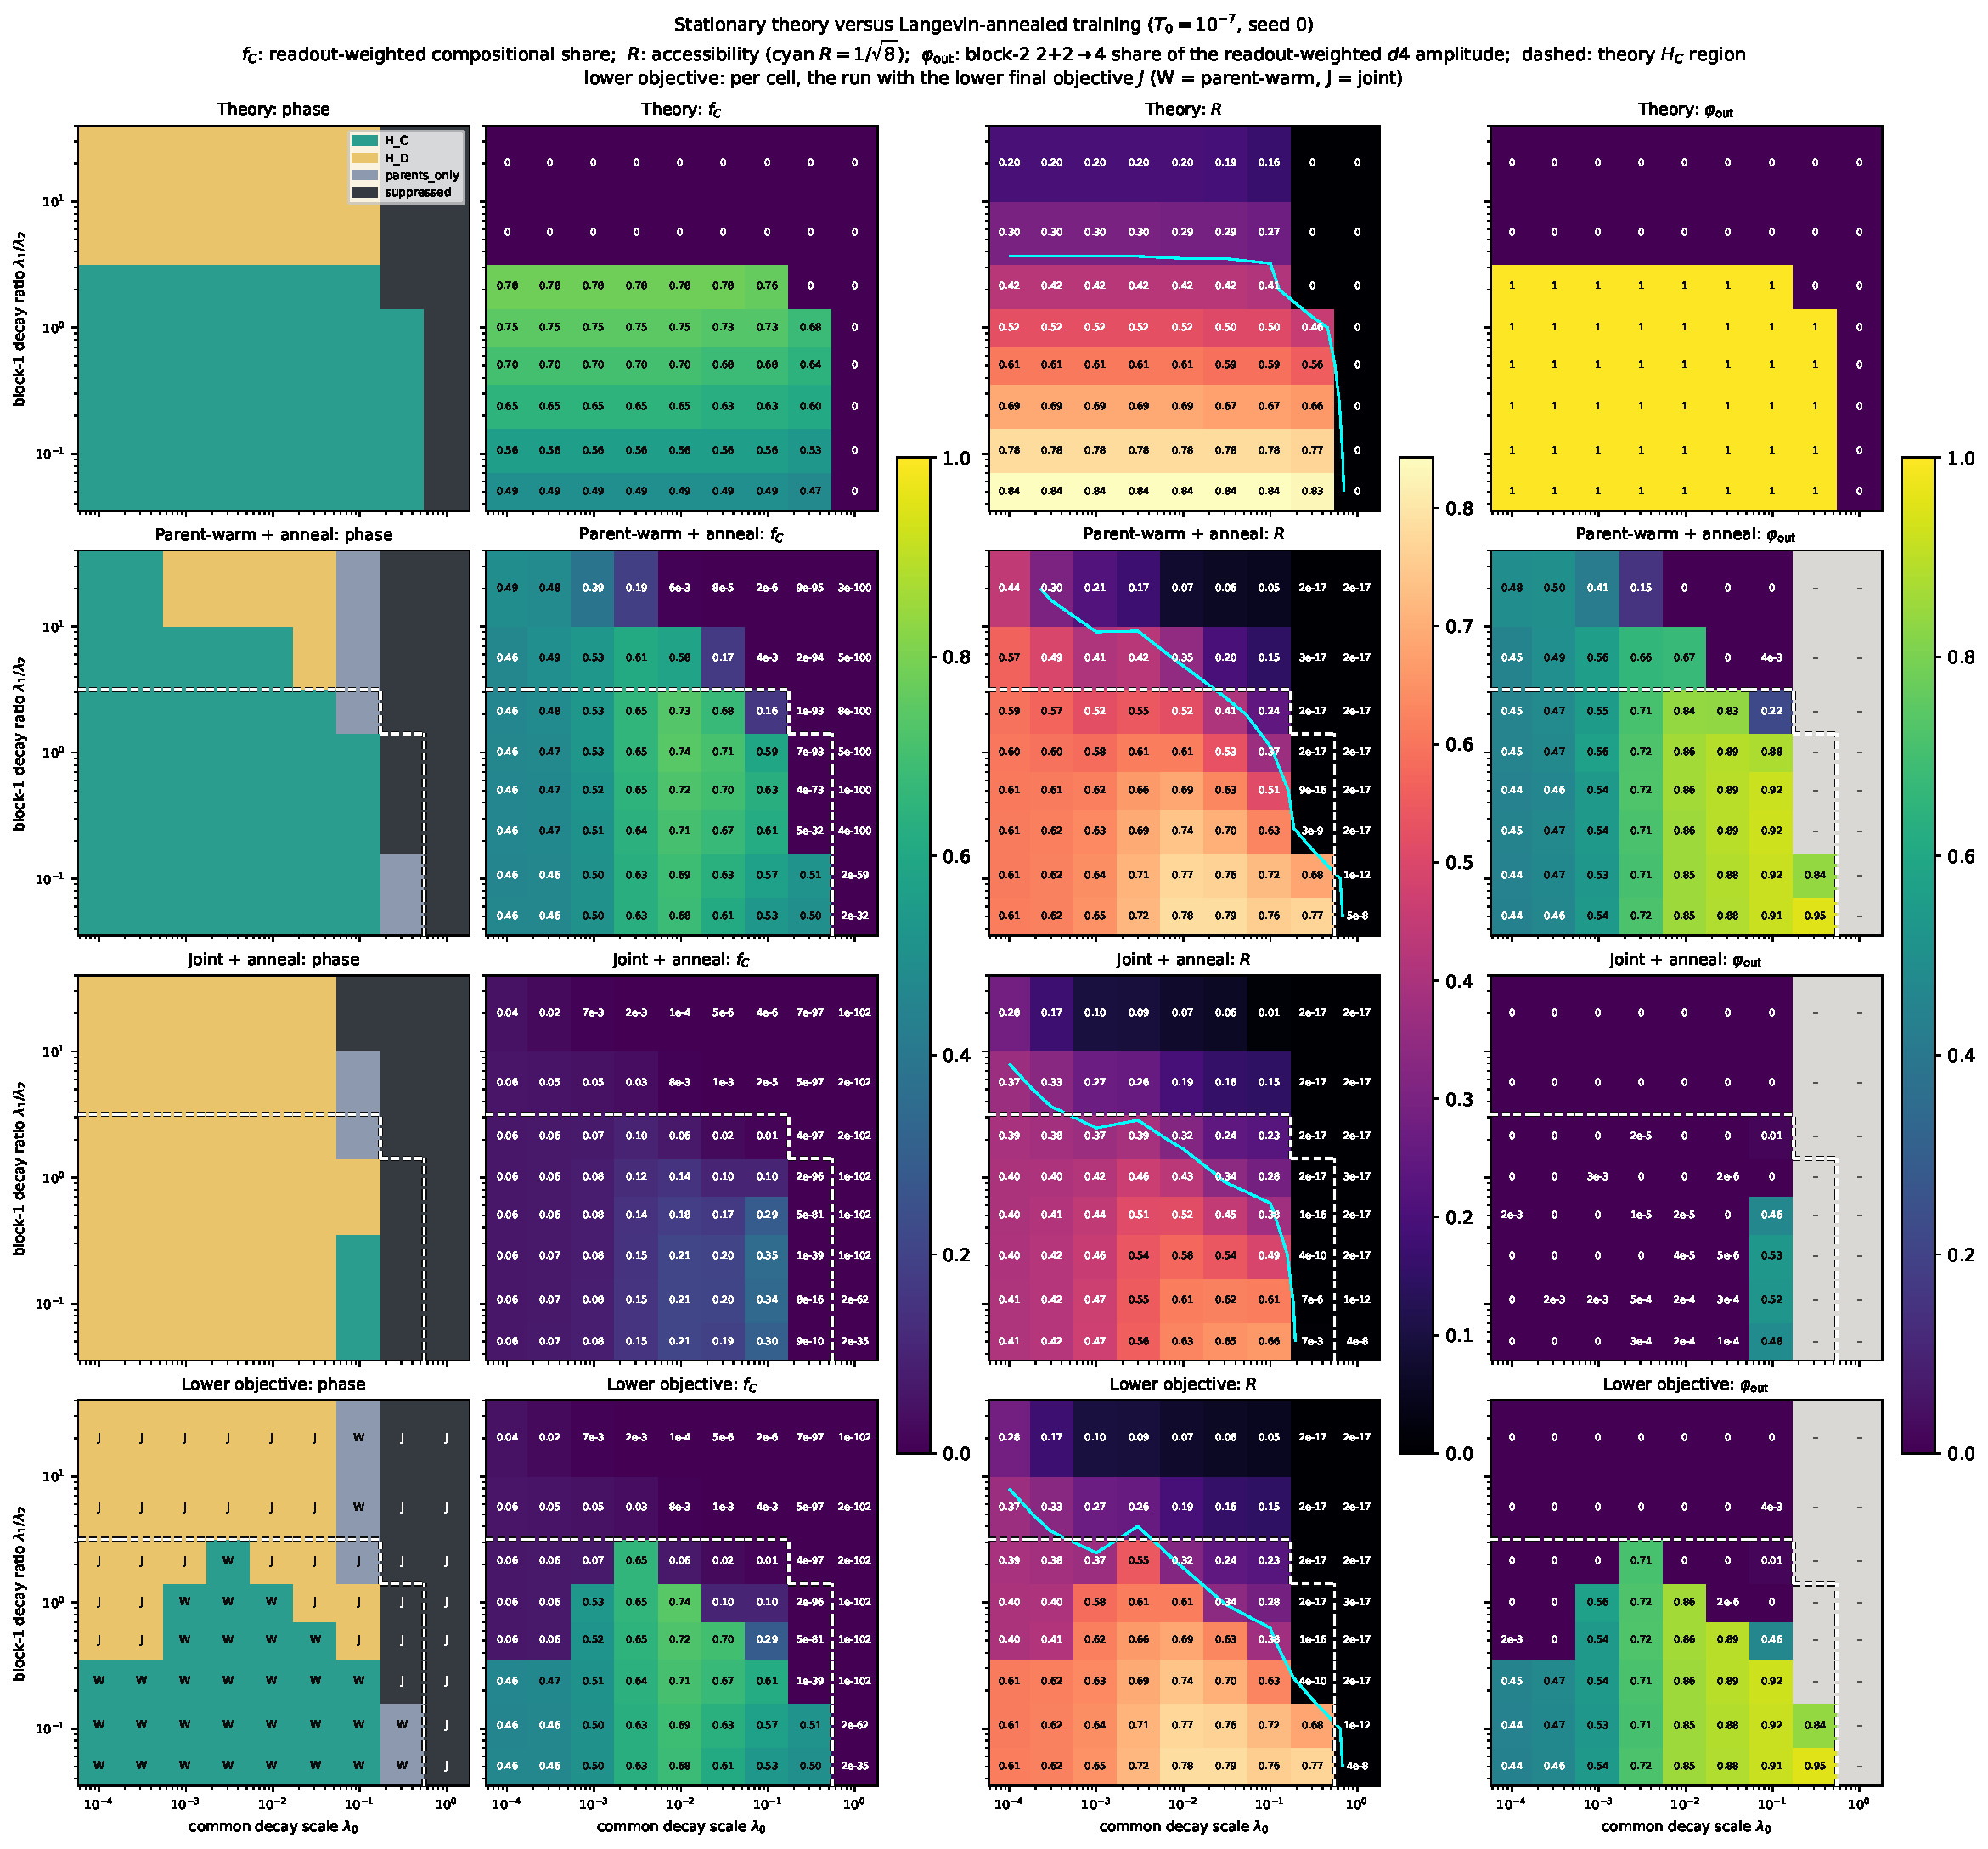
\includegraphics[width=\textwidth]{fig1_theory_vs_annealed.pdf}
\caption{\textbf{Theory, parent-warm + anneal, joint + anneal, and the lower-objective run per
cell (rows, top to bottom).}  In the bottom row each cell shows whichever of the two annealed runs
ended with the lower final objective $J$ (W = parent-warm, J = joint).  Columns: phase,
readout-weighted compositional share $f_C$, accessibility $R$ (cyan: $R=1/\sqrt8$), and the block-2
$2{+}2{\to}4$ share $\varphi_{\rm out}$ of the readout-weighted $d4$ amplitude.  Dashed: theory $H_C$
region.  Grey: no target mode produced (collapsed network).}
\end{figure}

\begin{figure}[p]
\centering
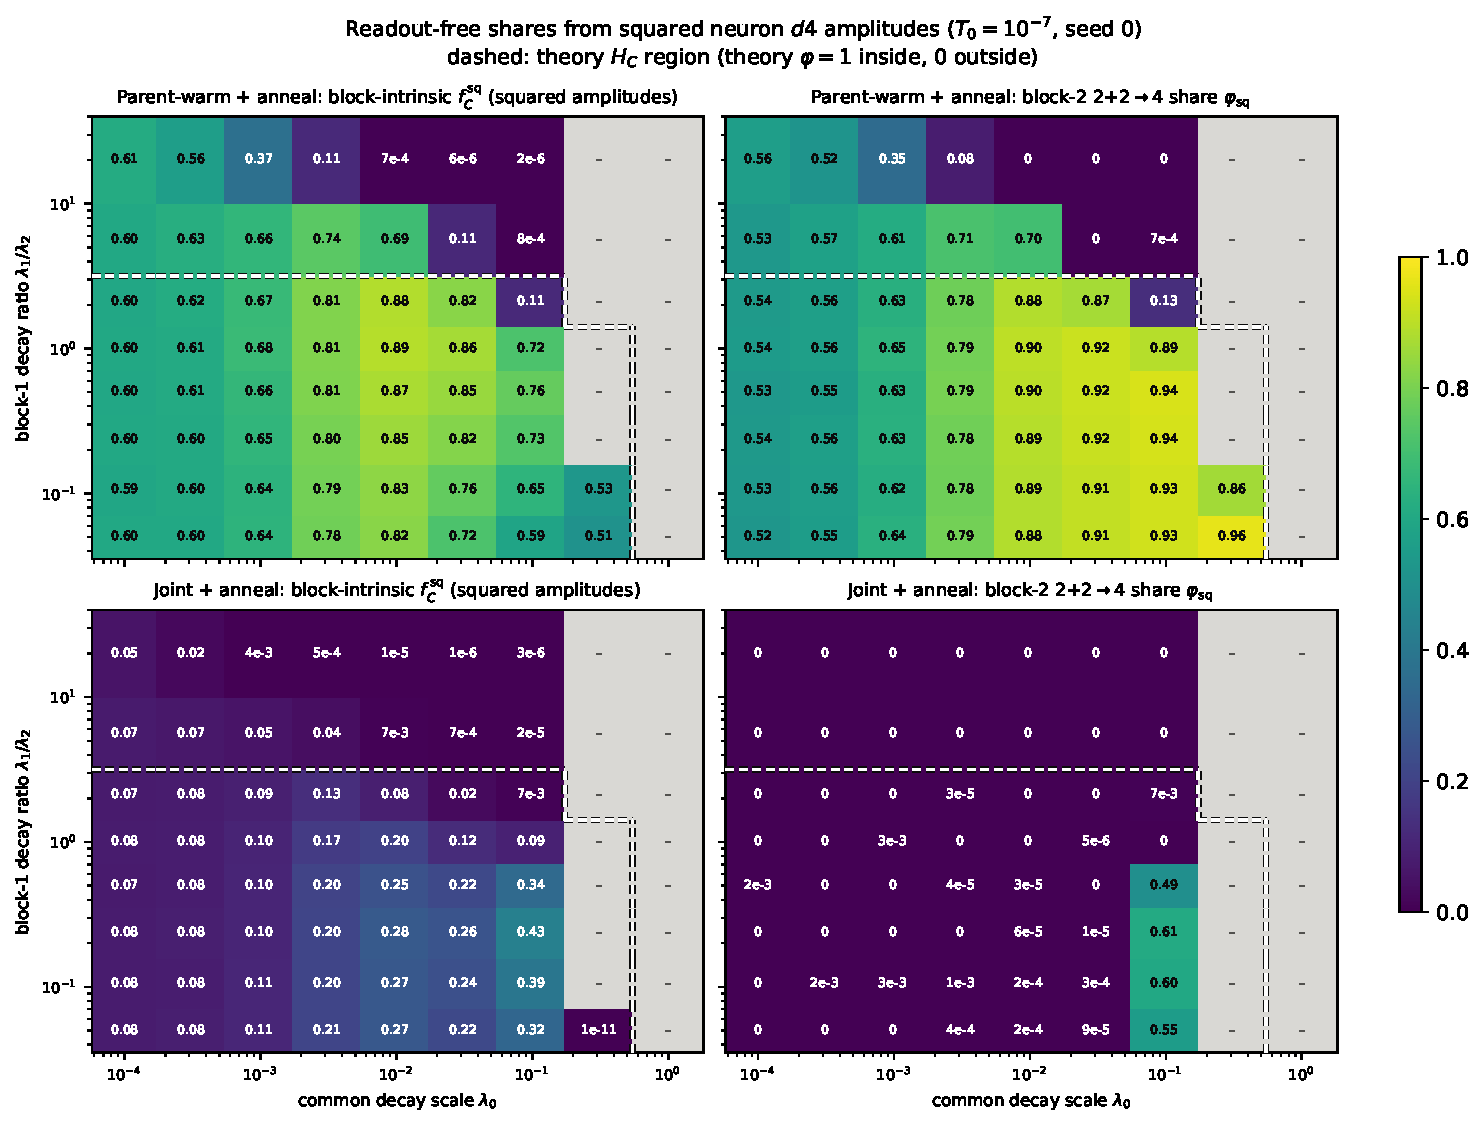
\includegraphics[width=0.78\textwidth]{fig2_block_intrinsic_shares.pdf}
\caption{\textbf{Readout-free shares} from squared neuron $d4$ amplitudes: $f_C^{\rm sq}$ (left)
and $\varphi_{\rm sq}$ (right); compare with columns 2 and 4 of Fig.~1.}
\vspace{6pt}
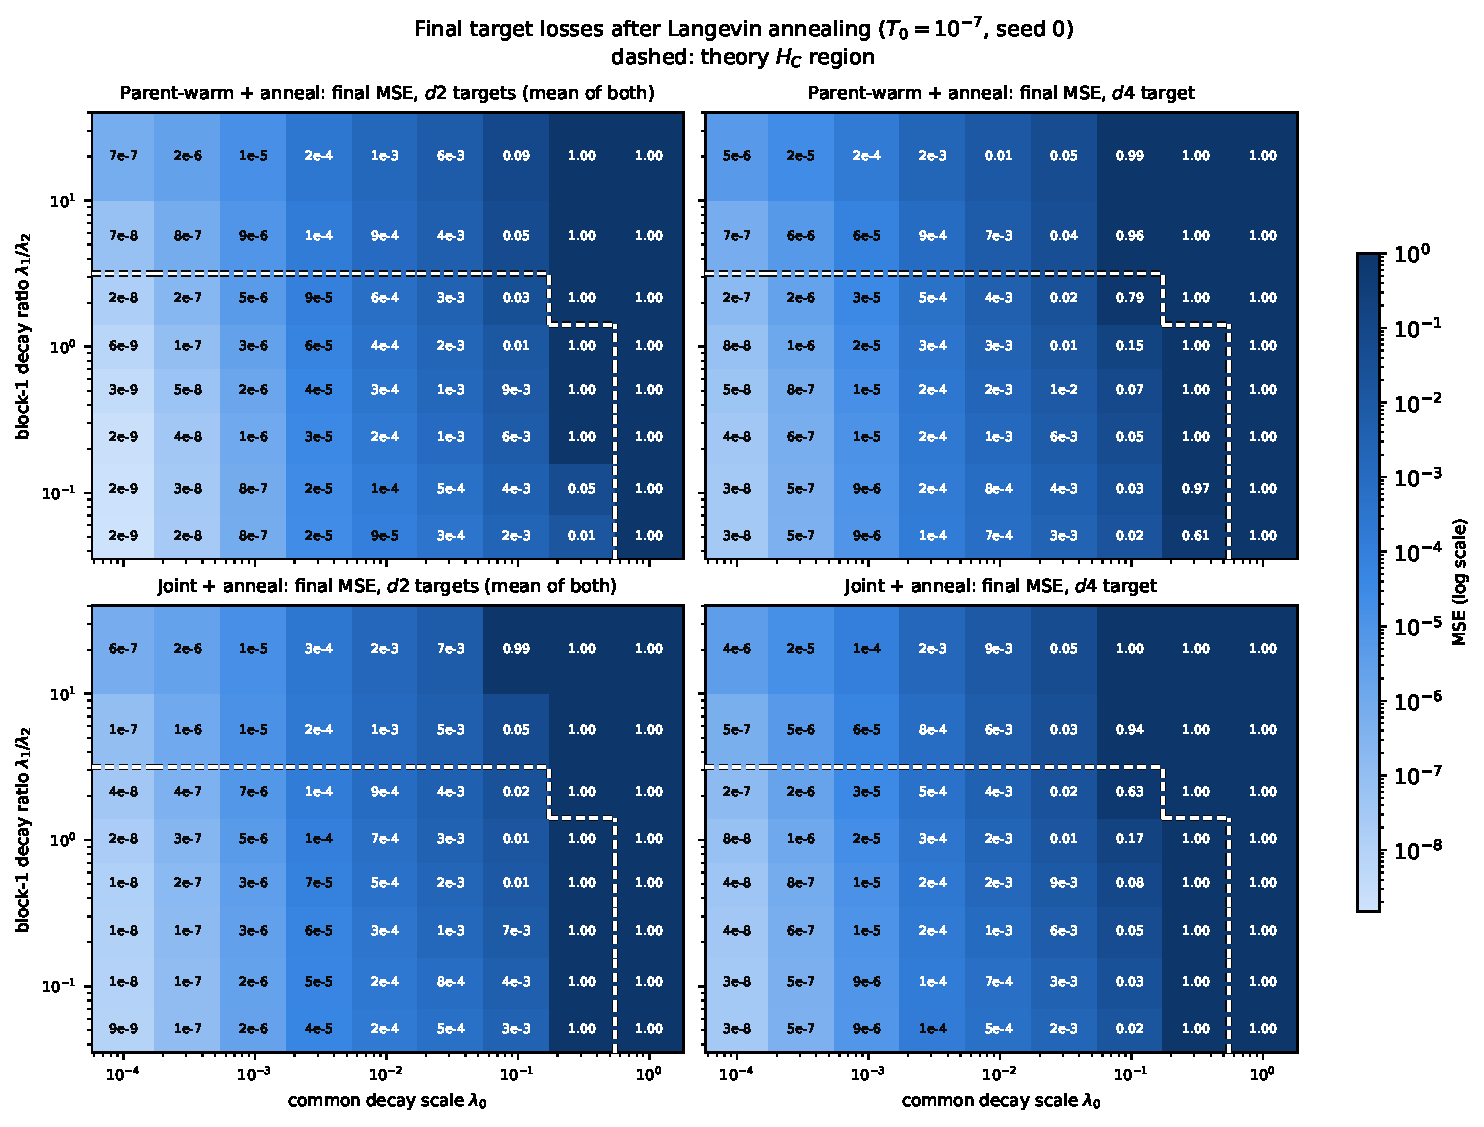
\includegraphics[width=0.78\textwidth]{fig3_final_mse.pdf}
\caption{\textbf{Final target losses:} MSE of the two $d2$ targets (mean) and of the $d4$ target,
log scale.}
\end{figure}

\end{document}
